% asset_id: AS1QuadraticsTikZ-004
% source: CCEA AS1-AF-LO005 + completing-the-square and maxima/minima evidence
% related_section: Core Theory Part B and Core Theory Part E
% purpose: Vertex form diagram for y = a(x-h)^2 + k and turning point (h,k).
\documentclass[tikz,border=8pt]{standalone}
\usetikzlibrary{arrows.meta,decorations.pathreplacing}
\begin{document}
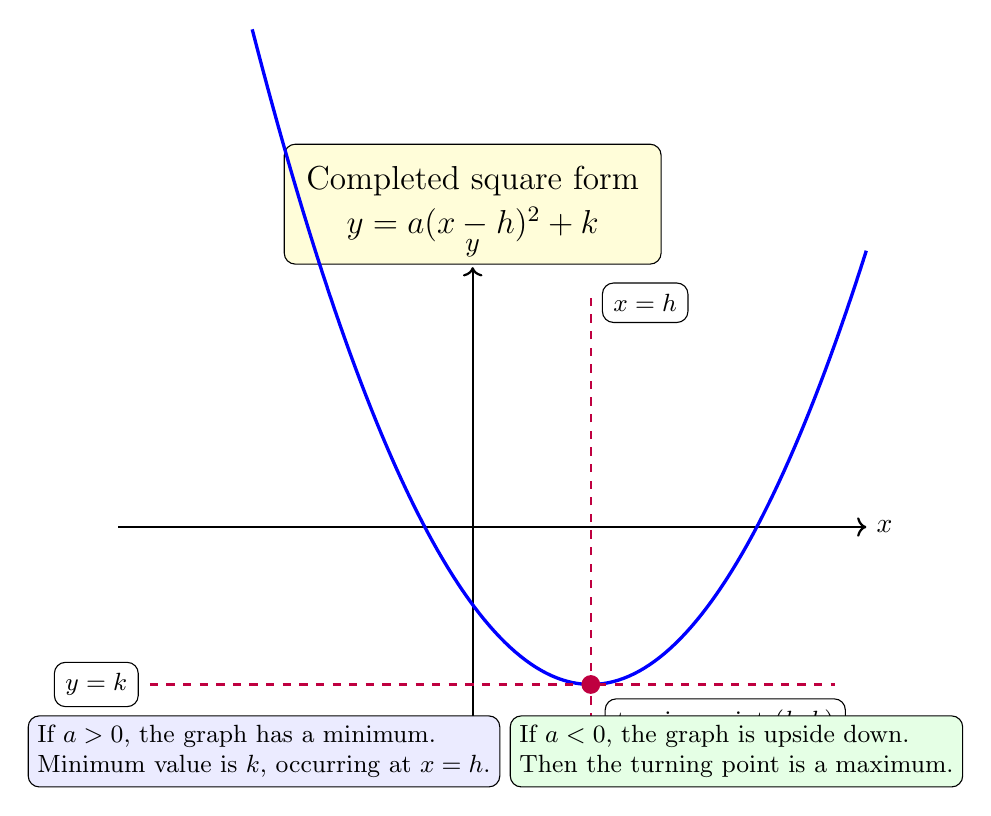
\begin{tikzpicture}[axis/.style={->, thick},curve/.style={very thick, blue},guide/.style={dashed, thick, purple},point/.style={circle, fill=purple, inner sep=2.4pt},labelbox/.style={draw, rounded corners, fill=white, inner sep=4pt, font=\small},formula/.style={draw, rounded corners, fill=yellow!15, inner sep=8pt, align=center, font=\large}]
\node[formula] at (0,4.1) {Completed square form\\[2pt]$y=a(x-h)^2+k$};
\draw[axis] (-4.5,0) -- (5,0) node[right] {$x$}; \draw[axis] (0,-3.3) -- (0,3.3) node[above] {$y$};
\draw[curve, domain=-2.8:5, samples=120] plot (\x,{0.45*(\x-1.5)*(\x-1.5)-2});
\coordinate (V) at (1.5,-2); \node[point] at (V) {}; \node[labelbox, below right=5pt] at (V) {turning point $(h,k)$};
\draw[guide] (1.5,-3.1) -- (1.5,3.0); \draw[guide] (-4.1,-2) -- (4.6,-2);
\node[labelbox, above right=4pt] at (1.5,2.45) {$x=h$}; \node[labelbox, left=4pt] at (-4.1,-2) {$y=k$};
\node[draw, rounded corners, fill=blue!8, align=left, font=\small] at (-2.65,-2.85) {If $a>0$, the graph has a minimum.\\Minimum value is $k$, occurring at $x=h$.};
\node[draw, rounded corners, fill=green!10, align=left, font=\small] at (3.35,-2.85) {If $a<0$, the graph is upside down.\\Then the turning point is a maximum.};
\end{tikzpicture}
\end{document}
